%!TEX root = ../../book_ML.tex
\chapter{Phân tích biệt thức tuyến tính}
\index{phân tích biệt thức tuyến tính -- linear discriminant analysis}
\index{LDA}
\section{Giới thiệu}
Trong chương trước, chúng ta đã làm quen với một thuật toán giảm chiều dữ liệu
phổ biến nhất  --  phân tích thành phần chính (PCA). Như đã đề cập, PCA là một thuật toán học không giám sát, tức chỉ sử dụng các vector dữ liệu mà
không cần tới nhãn. Tuy nhiên, trong bài toán phân loại,
việc khai thác mối liên quan giữa dữ liệu và nhãn sẽ mang lại kết quả phân loại
tốt hơn.
 
% ******************************************************************************
\begin{figure}[t]
\centering
    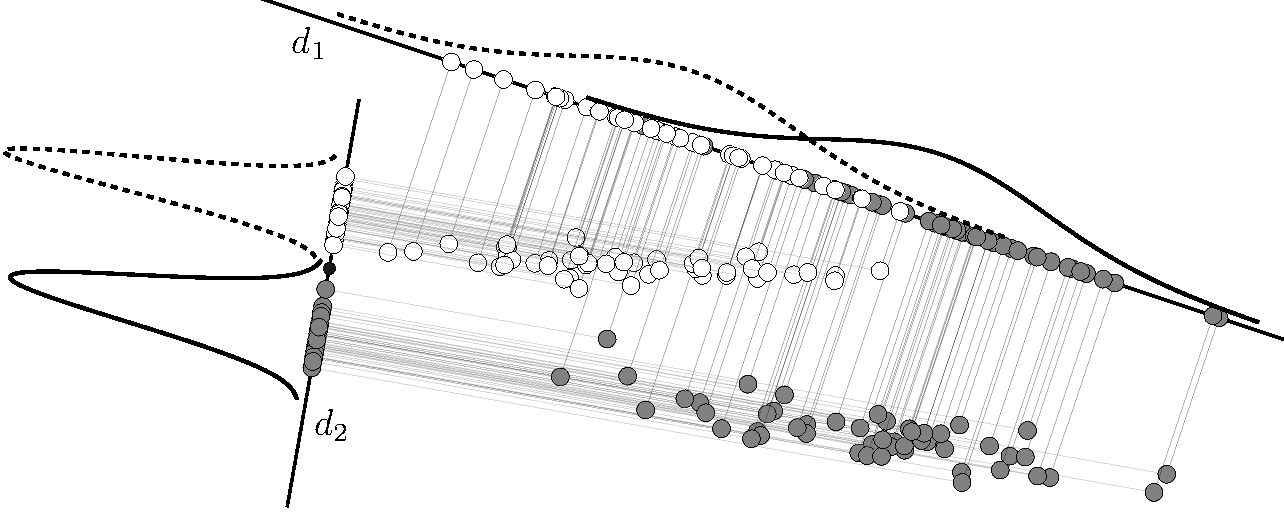
\includegraphics[width = \textwidth]{Chapters/07_DimemsionalityReduction/29_lda/latex/lda.pdf}
    \caption[]{Chiếu dữ liệu lên các đường thẳng khác nhau. Có hai lớp dữ liệu
    minh hoạ bởi các điểm màu xám và trắng trong không gian hai chiều. Số chiều
    được giảm về một bằng cách chiếu dữ liệu lên các đường thẳng khác nhau $d_1$
    và $d_2$. Trong hai cách chiếu này, phương của $d_1$ gần giống với phương
    của thành phần chính thứ nhất của dữ liệu, phương của $d_2$ gần với thành
    phần phụ của dữ liệu nếu dùng PCA. Khi chiếu dữ liệu lên $d_1$, nhiều điểm
    màu xám và trắng bị chồng lấn lên nhau, khiến cho việc phân loại dữ liệu là
    không khả thi trên đường thẳng này. Ngược lại, khi được chiếu lên $d_2$, dữ
    liệu của hai lớp được chia thành các cụm tương ứng tách biệt nhau, khiến cho
    việc phân loại trở nên đơn giản và hiệu quả hơn. Các đường cong hình
    chuông thể hiện xấp xỉ phân bố xác suất của dữ liệu hình chiếu trong mỗi
    lớp.}
    \label{fig:29_1}
\end{figure}
% ******************************************************************************
 
Nhắc lại rằng PCA là phương pháp giảm chiều dữ liệu sao cho lượng thông tin về
dữ liệu giữ lại, thể hiện ở tổng phương sai của các thành phần giữ lại, 
 là nhiều nhất. Tuy nhiên, trong nhiều bài toán, ta không cần giữ lại lượng
thông tin lớn nhất mà chỉ cần giữ lại thông tin cần thiết cho riêng bài toán đó. 
Xét ví dụ bài toán phân loại nhị phân được minh họa trong Hình~\ref{fig:29_1}. %
Ở đây, giả sử rằng dữ liệu được chiếu lên một đường thẳng và mỗi điểm được
thay bởi hình chiếu của nó lên đường thẳng kia. Như vậy, số chiều dữ liệu đã
được giảm từ hai về một. Câu hỏi đặt ra là đường thẳng cần có phương như thế
nào để hình chiếu của dữ liệu {có ích cho việc
phân loại nhất}? Việc phân loại trong không gian một chiều có thể hiểu là việc tìm ra một
ngưỡng giúp phân tách hai lớp. Xét hai
đường thằng $d_1$ và $d_2$. Trong đó phương của $d_1$ gần với phương của thành
phần chính nếu thực hiện PCA, phương của $d_2$ gần với phương của thành phần phụ
tìm được bằng PCA. Nếu thực hiện giảm chiều dữ liệu bằng PCA, ta sẽ thu được dữ
liệu gần với các điểm được chiếu lên $d_1$. Lúc này việc phân tách hai lớp trở
nên phức tạp vì các điểm dữ liệu mới của hai lớp chồng lấn lên nhau. Ngược lại,
nếu ta chiếu dữ liệu lên đường thẳng gần với thành phần phụ tìm được bởi PCA,
tức $d_2$, các điểm hình chiếu nằm hoàn toàn về hai phía khác nhau của điểm màu
đen trên đường thẳng này. Như vậy, việc chiếu dữ liệu lên $d_2$ sẽ mang lại hiệu
quả hơn trong bài toán phân loại. Việc phân loại một điểm dữ liệu mới được xác
định nhanh chóng bằng cách so sánh hình chiếu của nó lên $d_2$ với điểm phân ngưỡng màu đen.

Qua ví dụ trên ta thấy rằng, {việc giữ lại thông tin nhiều nhất không mang lại
kết quả tốt trong một số trường hợp.} Chú ý rằng kết quả của phân tích trên
đây không có nghĩa là thành phần phụ mang lại hiệu quả tốt
hơn thành phần chính. Việc chiếu dữ liệu lên đường thẳng
nào giúp ích cho các bài toán phân loại cần nhiều phân tích cụ thể hơn.
Ngoài ra, hai đường thằng $d_1$ và $d_2$ trên đây không vuông góc với nhau,
chúng được chọn gần với các thành phần chính và phụ của dữ liệu phục vụ cho mục
đích minh hoạ. 

% \index{LDA}
\index{ma trận chiếu -- projection matrix}
\index{biệt thức -- discriminant}
\textit{Phân tích biệt thức tuyến tính} (linear discriminant analysis, LDA) ra đời giúp tìm phương chiếu dữ liệu
hiệu quả cho bài toán phân loại. LDA có thể được coi là một phương pháp giảm
chiều dữ liệu hoặc phân loại, hoặc
được áp dụng đồng thời cho cả hai, tức giảm chiều dữ liệu sao cho việc phân loại
hiệu quả nhất. Số chiều của dữ liệu mới nhỏ hơn hoặc bằng $C-1$ trong đó $C$
là số lớp dữ liệu. Từ \textit{biệt thức} ({discriminant}) được hiểu là \textit{những
thông tin riêng biệt của mỗi lớp}. 
  
Trong Mục~\ref{sec:29_2} dưới đây, chúng ta sẽ thảo luận về LDA cho bài toán
phân loại nhị phân. Mục~\ref{sec:29_3} sẽ tổng quát LDA lên cho trường hợp phân
loại đa lớp. Mục~\ref{sec:29_4} trình bày các ví dụ và mã nguồn Python cho LDA.
 
 
\section{Bài toán phân loại nhị phân}
\label{sec:29_2}
\subsection{Ý tưởng cơ bản}
\index{do@độ lệch chuẩn -- standard deviation}
Quay lại với Hình~\ref{fig:29_1}, giả sử dữ liệu của mỗi lớp khi chiếu
xuống một đường thẳng tuân theo phân phối chuẩn có hàm mật độ xác suất dạng hình chuông. Độ rộng của mỗi đường hình chuông này thể hiện \textit{độ lệch
chuẩn} ({standard deviation}\footnote{độ lệch chuẩn là căn bậc hai của
phương sai}, ký hiệu là $s$) của dữ liệu. Dữ liệu càng tập trung thì độ lệch
chuẩn càng nhỏ,
càng phân tán thì độ lệch chuẩn càng cao. Khi chiếu lên $d_1$, dữ liệu của
hai lớp bị phân tán quá nhiều và trộn lẫn vào nhau. Khi chiếu lên $d_2$, mỗi lớp
có độ lệch chuẩn nhỏ, khiến dữ liệu trong từng
lớp tập trung hơn. 
 

Tuy nhiên, việc độ lệch chuẩn nhỏ trong mỗi lớp chưa đủ để đảm bảo độ độ riêng
biệt của dữ liệu giữa hai lớp. Xét các ví dụ trong
Hình~\ref{fig:29_2}. Hình \ref{fig:29_2}a thể hiện trường hợp 
dữ liệu được chiếu lên $d_1$ như trong Hình~\ref{fig:29_1}. Cả hai lớp đều quá
phân 
tán khiến lượng chồng lấn lớn (phần diện tích màu xám), tức dữ liệu chưa
thực sự riêng biệt. Hình \ref{fig:29_2}b thể hiện trường hợp độ lệch
chuẩn của hai lớp đều nhỏ, tức dữ liệu trong mỗi lớp tập trung hơn. Tuy nhiên, khoảng cách giữa hai lớp, được đo bằng khoảng cách
giữa hai trung bình $m_1$ và $m_2$ là quá nhỏ. Việc này khiến phần chồng lấn chiếm
môt tỉ lệ lớn, không tốt cho việc phân loại.
Hình~\ref{fig:29_2}c thể hiện trường hợp cả hai độ lệch chuẩn nhỏ và khoảng
cách giữa hai trung bình lớn, phần chồng lấn nhỏ không đáng kể.
 
Vậy, độ lệch chuẩn và khoảng cách giữa hai trung bình cụ thể đại diện cho các tiêu
chí gì? 
\index{phương sai nội lớp -- within-class variance}
\index{phương sai liên lớp -- between-class variance}
\begin{itemize}
    \item Độ lệch chuẩn nhỏ thể hiện việc dữ liệu ít phân tán, tức dữ liệu
    trong mỗi lớp có xu hướng giống nhau. Hai phương sai $s_1^2, s_2^2$ còn được
    gọi là các \textit{phương sai nội lớp} ({within-class variance}).
     
    \item Khoảng cách giữa các trung bình lớn chứng tỏ hai lớp cách xa
    nhau, tức dữ liệu giữa hai lớp khác nhau nhiều. Bình phương khoảng cách
    giữa hai trung bình $(m_1 - m_2)^2$ còn được gọi là \textit{phương sai liên lớp} ({between-class variance}). Ở đây bình phương của hiệu hai trung bình được lấy để có cùng thứ nguyên với phương sai.
\end{itemize}
 
% ******************************************************************************
\begin{figure}[t]
    \centering
        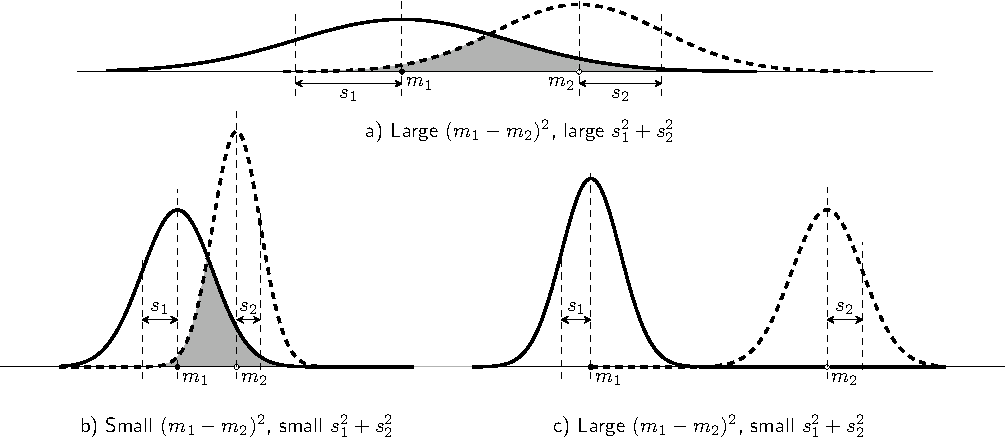
\includegraphics[width = \textwidth]{Chapters/07_DimemsionalityReduction/29_lda/latex/lda4.pdf}
        \caption[]{Khoảng cách giữa các trung bình và tổng các phương sai ảnh hưởng
        tới độ biệt thức của dữ liệu. (a) Khoảng cách giữa hai trung bình
        lớn nhưng phương sai trong mỗi class cũng lớn, khiến cho hai phân phối
        chồng lấn lên nhau (phần màu xám). (b) Phương sai cho mỗi class rất nhỏ
        nhưng hai trung bình quá gần nhau, khiến khó phân biệt hai class. (c) Khi
        phương sai đủ nhỏ và khoảng cách giữa hai trung bình đủ lớn, ta thấy rằng dữ
        liệu hai lớp tách biệt hơn.}
        \label{fig:29_2}
   \end{figure} 
   % ******************************************************************************
Hai lớp dữ liệu được gọi là {tách biệt} (discriminative) nếu hai lớp đó cách xa nhau
(phương sai liên lớp lớn) và dữ liệu trong mỗi lớp có xu hướng giống nhau
(phương sai nội lớp nhỏ). LDA là thuật toán đi tìm một phép chiếu sao cho tỉ
lệ giữa phương sai liên lớp và phương sai nội lớp trở nên lớn
nhất có thể.
 
 
\subsection{Hàm mục tiêu của phân tích biệt thức tuyến tính}
Giả sử có $N$ điểm dữ liệu $\mathbf{x}_1, \mathbf{x}_2, \dots,
\mathbf{x}_N \in \R^D$ trong đó $N_1 < N$ điểm đầu tiên thuộc lớp thứ nhất,
$N_2 = N - N_1$ điểm còn lại thuộc lớp thứ hai. Ký hiệu $\mathcal{C}_1 = \{n | 1
\leq n \leq N_1\}$ là tập hợp chỉ số các điểm thuộc lớp thứ nhất và
$\mathcal{C}_2 = \{m| N_1 + 1 \leq m \leq N\})$ là tập hợp  chỉ số các
điểm thuộc lớp thứ hai. Phép chiếu dữ liệu xuống một đường thẳng được mô
tả bằng một vector trọng số $\mathbf{w}$, giá trị tương ứng của mỗi điểm dữ liệu
chiếu được cho bởi
\begin{equation} 
z_n = \mathbf{w}^T\mathbf{x}_n, 1 \leq n \leq N.
\end{equation} 
Vector trung bình của mỗi lớp được tính bởi  
\begin{eqnarray} 
\label{eqn:29_1}
\mathbf{m}_k &=& \frac{1}{N_k}\sum_{n \in \mathcal{C}_k}\mathbf{x}_n,~~~ k = 1,
2 \\
\label{eqn:29_2}
\imply m_1 - m_2 &=& \frac{1}{N_1}\sum_{i \in \mathcal{C}_1}z_i -
\frac{1}{N_2}\sum_{j \in \mathcal{C}_2}z_j =  \mathbf{w}^T(\mathbf{m}_1 - \mathbf{m}_2).
\end{eqnarray} 
Các phương sai nội lớp được định nghĩa bởi
\begin{equation} 
\label{eqn:29_3}
s_k^2 = \sum_{n \in \mathcal{C}_k} (z_n - m_k)^2, ~~ k = 1, 2 
\end{equation} 
\textit{Chú ý:} Các phương sai nội lớp không được lấy trung bình như
phương sai thông thường. Điều này có thể lý giải bởi tầm quan trọng của mỗi
phương sai nội lớp cần tỉ lệ thuận với số lượng điểm dữ liệu trong lớp đó,
tức phương sai nội lớp bằng phương sai nhân với số điểm trong lớp đó.
 
LDA là thuật toán đi tìm giá trị lớn nhất của hàm mục tiêu:
\begin{equation} 
\label{eqn:29_4}
    J(\mathbf{w}) = \frac{(m_1 - m_2)^2}{s_1^2 + s_2^2}
\end{equation} 
Thông qua việc tối đa hàm mục tiêu này, ta sẽ thu được phương sai liên lớp $(m_1 - m_2)^2$ lớn và phương sai nội lớp $s_1^2 + s_2^2$
nhỏ.

Tiếp theo, chúng ta sẽ tìm biểu thức phụ thuộc giữa tử số và mẫu số trong vế
phải của~\eqref{eqn:29_4} vào $\mathbf{w}$. Tử số được viết lại thành:
\begin{eqnarray*} 
    \label{eqn:29_5}
    (m_1 - m_2)^2 = (\bw^T(\bm_1 - \bm_2))^2 = \mathbf{w}^T
    \underbrace{(\mathbf{m}_1 - \mathbf{m}_2)(\mathbf{m}_1 - \mathbf{m}_2)^T}_{\mathbf{S}_B} \mathbf{w} = \mathbf{w}^T\mathbf{S}_B \mathbf{w}
\end{eqnarray*} 
\index{ma trận phương sai liên lớp -- between-class variance matrix}
\index{ma trận phương sai nội lớp -- within-class variance matrix}

$\mathbf{S}_B$ còn được gọi là \textit{ma trận phương sai liên lớp}. Có
thể thấy đây là một ma trận đối xứng nửa xác định dương. 

Mẫu số được viết lại thành:
\begin{eqnarray} 
    \nonumber
    s_1^2 + s_2^2 &=& \sum_{k=1}^2 \sum_{n \in \mathcal{C}_k} \left(\mathbf{w}^T(\mathbf{x}_n - \mathbf{m}_k)\right)^2 \\\ 
    \label{eqn:29_6}
    &=&\mathbf{w}^T \underbrace{\sum_{k=1}^2 \sum_{n \in \mathcal{C}_k} (\mathbf{x}_n - \mathbf{m}_k)(\mathbf{x}_n - \mathbf{m}_k)^T}_{\mathbf{S}_W} \mathbf{w} = \mathbf{w}^T\mathbf{S}_W \mathbf{w}
\end{eqnarray} 
$\mathbf{S}_W$ còn được gọi là \textit{ma trận phương sai nội lớp}. Đây
là một ma trận đối xứng nửa xác định dương vì nó là tổng của hai ma trận
đối xứng nửa xác định dương\footnote{\begin{math} 
(\mathbf{a}^T\mathbf{b})^2 = (\mathbf{a}^T\mathbf{b})(\mathbf{a}^T\mathbf{b}) = \mathbf{a}^T\mathbf{b}\mathbf{b}^T\mathbf{a} 
\end{math} 
với $\mathbf{a}, \mathbf{b}$ là hai vector cùng chiều bất kỳ. }.
 
Như vậy, bài toán tối ưu cho LDA trở thành
\begin{equation} 
\label{eqn:29_7}
\mathbf{w}  = \arg\max_{\mathbf{w}}\frac{\mathbf{w}^T\mathbf{S}_B \mathbf{w}}{\mathbf{w}^T\mathbf{S}_W\mathbf{w}}
\end{equation} 
 
 
 
\subsection{Nghiệm của bài toán tối ưu}
Nghiệm $\mathbf{w}$ của \eqref{eqn:29_7} là nghiệm của phương trình đạo hàm
hàm mục tiêu bằng không. Sử dụng quy tắc chuỗi cho đạo hàm  nhiều biến và công
thức $\nabla_{\mathbf{w}}\mathbf{w} \mathbf{A}\mathbf{w} = 2\mathbf{Aw}$ với
$\mathbf{A}$ là một ma trận đối xứng, ta thu được: 
\begin{eqnarray} 
    \label{eqn:29_8}
    \nabla_{\mathbf{w}} J(\mathbf{w}) &=& \frac{1}{(\mathbf{w}^T\mathbf{S}_{W}\mathbf{w})^2} \left( 
    2\mathbf{S}_B \mathbf{w} (\mathbf{w}^T\mathbf{S}_{W}\mathbf{w}) - 2\mathbf{w}^T\mathbf{S}_{B}\mathbf{w}^T\mathbf{S}_W \mathbf{w} 
    \right) = \mathbf{0}\\\ 
    \label{eqn:29_9}
    \Leftrightarrow \mathbf{S}_B\mathbf{w} &=& \frac{\mathbf{w}^T\mathbf{S}_B
    \mathbf{w}}{\mathbf{w}^T\mathbf{S}_W\mathbf{w}}\mathbf{S}_W\mathbf{w} =
    J(\bw)\bS_W\bw\\\
    \label{eqn:29_10}
    \imply \mathbf{S}_W^{-1}\mathbf{S}_B \mathbf{w} &=& J(\mathbf{w})\mathbf{w}
\end{eqnarray} 
\textbf{Lưu ý:} Trong~\eqref{eqn:29_10}, ta đã giả sử rằng ma trận
$\mathbf{S}_W$ khả nghịch. Điều này không luôn đúng, nhưng có thể được khắc phục bằng một kỹ
thuật nhỏ là xấp xỉ $\mathbf{S}_W$ bởi $ \bar{\mathbf{S}}_W =
\mathbf{S}_W + \lambda\mathbf{I}$ với $\lambda$ là một số thực dương nhỏ. Ma
trận mới này khả nghịch vì trị riêng nhỏ nhất của nó dương, bằng với trị riêng nhỏ
nhất của $\mathbf{S}_W$ cộng với $\lambda$. Điều
này suy ra từ việc $\mathbf{S}_W$ là một ma trận nửa xác định dương. Từ đó,
$\bar{\mathbf{S}}_W$ là một ma trận xác định dương vì mọi trị riêng của nó không nhỏ hơn $\lambda$, và vì vậy khả nghịch. Khi tính toán, ta có thể sử
dụng nghịch đảo của $\bar{\mathbf{S}}_W$. Kỹ thuật này được sử dụng rất nhiều
khi cần sử dụng nghịch đảo của một ma trận nửa xác định dương và chưa biết nó có
thực sự xác định dương hay không.
 
% \index{Fisher's linear discriminant}
Trở lại đẳng thức~\eqref{eqn:29_10}, vì $J(\mathbf{w})$ là một số vô
hướng, ta suy ra $\mathbf{w}$ phải là một vector riêng của
$\mathbf{S}_W^{-1}\mathbf{S}_B$ ứng với $J(\mathbf{w})$. Vậy, để hàm mục tiêu là
lớn nhất thì $J(\mathbf{w})$ phải là trị riêng lớn nhất của
$\mathbf{S}_W^{-1}\mathbf{S}_B$. Dấu bằng xảy ra khi $\mathbf{w}$ là vector
riêng ứng với trị riêng lớn nhất đó. 
Từ đó, nếu $\mathbf{w}$ là nghiệm của \eqref{eqn:29_7} thì
$k\mathbf{w}$ cũng là nghiệm với $k$ là số thực khác không bất kỳ. Vậy ta có thể
chọn $\mathbf{w}$ sao cho $(\mathbf{m}_1 - \mathbf{m}_2)^T\mathbf{w} =  L$ với
$L$ là trị riêng lớn nhất của $\mathbf{S}_W^{-1}\mathbf{S}_B$ và cũng là giá
trị tối ưu của $J(\bw)$. Khi đó, thay định nghĩa của $\mathbf{S}_B$ ở
\eqref{eqn:29_5} vào \eqref{eqn:29_10} ta có:
\begin{equation} 
L \mathbf{w} = \mathbf{S}_{W}^{-1}(\mathbf{m}_1 - \mathbf{m}_2)\underbrace{(\mathbf{m}_1 - \mathbf{m}_2)^T\mathbf{w}}_L =  L\mathbf{S}_{W}^{-1}(\mathbf{m}_1 - \mathbf{m}_2) 
\end{equation} 
Điều này nghĩa là ta có thể chọn
\begin{equation} 
\label{eqn:29_11}
\mathbf{w} = \alpha\mathbf{S}_{W}^{-1}(\mathbf{m}_1 - \mathbf{m}_2)
\end{equation} 
với $\alpha \neq 0$ bất kỳ. Biểu thức \eqref{eqn:29_11} còn được biết với tên gọi \textit{biệt thức tuyến tính Fisher}
({Fisher's linear discriminant}), được đặt theo tên nhà khoa học Ronald 
Fisher (\url{https://goo.gl/eUk1KS}).
 
\index{biệt thức tuyến tính Fisher -- Fisher's linear discriminant}
 
\section{Bài toán phân loại đa lớp}
\label{sec:29_3} 
 
\subsection{Xây dựng hàm mục tiêu}
\index{LDA đa lớp -- multi-class LDA}
Trong mục này, chúng ta sẽ xem xét trường hợp tổng quát của LDA khi có nhiều hơn hai lớp
dữ
liệu, $C > 2$. Giả sử rằng chiều của dữ liệu $D$ lớn hơn $C$.
Đặt số chiều dữ liệu mới là $D' < D$ và dữ liệu mới ứng với mỗi điểm dữ liệu $\mathbf{x}$ là: 
\begin{equation} 
\bz = \mathbf{W}^T\mathbf{x} 
\end{equation} 
với $\mathbf{W} \in \mathbb{R}^{D\times D'}$. 
\newpage
Một vài ký hiệu: 
\begin{itemize}
\item $\mathbf{X}_k, \mathbf{Z}_k = \mathbf{W}^T\mathbf{X}_k$ lần lượt là ma
trận dữ liệu của lớp thứ $k$ trong không gian ban đầu và không gian mới với số
chiều nhỏ hơn. Mỗi cột tương ứng với một điểm dữ liệu. 
 
\item $\displaystyle \mathbf{m}_k = \frac{1}{N_k}\sum_{n \in
\mathcal{C}_k}\mathbf{x}_k \in \mathbb{R}^{D}$ là vector trung bình của lớp $k$ trong không gian ban đầu.
 
\item $\displaystyle \mathbf{e}_k = \frac{1}{N_k}\sum_{n \in \mathcal{C}_k}
\bz_n = \mathbf{W}^T\mathbf{m}_k \in \mathbb{R}^{D'}$ là vector trung bình của lớp
$k$ trong không gian mới.
 
\item $\mathbf{m} \in \R^D$ là vector trung bình của toàn bộ dữ liệu trong không
gian ban đầu và $\mathbf{e} \in R^{D'}$ là vector trung bình trong không gian
mới.
\end{itemize}
 
 
%% *****************************************************************************
\begin{figure}[t]
     % caption on side     
     \floatbox[{\capbeside\thisfloatsetup{capbesideposition={right,top},capbesidewidth=6cm}}]{figure}[\FBwidth]
     {\caption{ LDA cho bài toán phân loại đa lớp. Mục đích chung là phương sai nội lớp nhỏ và phương sai liên lớp lớn. Các vòng tròn thể hiện các lớp khác nhau. }
     \label{fig:29_3}}
     { % figure here
     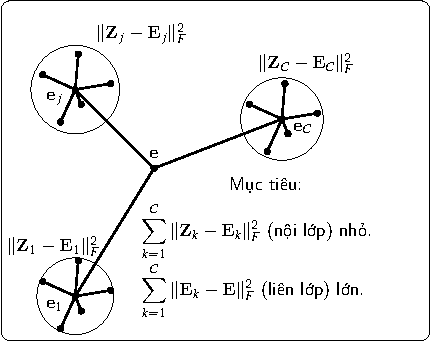
\includegraphics[width=.5\textwidth]{Chapters/07_DimemsionalityReduction/29_lda/latex/multi_LDA.pdf}
     }
\end{figure}
%% *****************************************************************************
Một trong những cách xây dựng hàm mục tiêu cho LDA đa lớp được minh họa
trong Hình~\ref{fig:29_3}. Độ phân tán của một lớp dữ liệu được coi
như tổng bình phương khoảng cách từ mỗi điểm trong lớp đó tới vector trung bình của chúng. Nếu
tất cả các điểm đều gần vector trung bình này thì tập dữ liệu đó có độ phân tán nhỏ. Ngược lại, nếu tổng này lớn, tức trung bình các điểm đều
xa trung tâm, tập hợp này được coi là có độ phân tán cao.
Dựa vào nhận xét này, ta có thể xây dựng các đại lượng phương sai nội lớp và liên lớp như sau đây. 

Phương sai nội lớp của lớp thứ $k$ được định nghĩa như sau:
\begin{eqnarray} 
    \label{eqn:29_15}
    \sigma_k^2 &=& \sum_{n \in \mathcal{C}_k} \|\bz_n -\mathbf{e}_k\|_F^2 = \|\mathbf{Z}_k - \mathbf{E}_k\|_2^2 
    = \|\mathbf{W}^T (\mathbf{X}_k - \mathbf{M}_k) \|_F^2\\\ 
    &=& \text{trace}\left(\mathbf{W}^T (\mathbf{X}_k - \mathbf{M}_k)(\mathbf{X}_k - \mathbf{M}_k)^T \mathbf{W}\right) 
\end{eqnarray} 
Với $\mathbf{E}_k$ là một ma trận có các cột giống hệt nhau và bằng với vector trung bình $\mathbf{e}_k$. Có thể nhận thấy $ \mathbf{E}_k =
\mathbf{W}^T\mathbf{M}_k$ với $\mathbf{M}_k$ là ma trận có các cột giống hệt
nhau và bằng với vector trung bình $\mathbf{m}_k$ trong không gian ban đầu. 
Vậy đại lượng đo phương sai nội lớp trong LDA đa lớp có thể được đo bằng: 
\begin{eqnarray} 
    \nonumber
    \label{eqn:29_17}
    s_W = \sum_{k = 1}^C \sigma_k^2 &=& \sum_{k=1}^C
    \text{trace}\left(\mathbf{W}^T (\mathbf{X}_k - \mathbf{M}_k)(\mathbf{X}_k - \mathbf{M}_k)^T \mathbf{W}\right) = \text{trace}\left( \mathbf{W}^T\mathbf{S}_W \mathbf{W}\right) 
\end{eqnarray} 
với
\begin{equation} 
    \label{eqn:29_19}
    \mathbf{S}_W = \sum_{k=1}^C \|\mathbf{X}_k- \mathbf{M}_k \|_F^2 = \sum_{k=1}^C \sum_{n \in \mathcal{C}_k} (\mathbf{x}_n - \mathbf{m}_k)(\mathbf{x}_n - \mathbf{m}_k)^T
\end{equation} 
Ma trận $\mathbf{S}_W$ này là một ma trận nửa xác định dương. 
 
 
Phương sai liên lớp lớn có thể đạt được nếu tất cả các điểm trong
không gian mới đều xa vector trung bình chung $\mathbf{e}$. Điều này cũng có thể
đạt được nếu các vector trung bình của mỗi lớp xa các vector trung bình chung
(trong không gian mới). Vậy ta có thể định nghĩa đại lượng phương sai liên lớp như sau:
\begin{equation} 
    \label{eqn:29_20}
    s_B = \sum_{k=1}^C N_k \|\mathbf{e}_k - \mathbf{e} \|_F^2 = \sum_{k=1}^C \|\mathbf{E}_k - \mathbf{E} \|_F^2
\end{equation} 
Ta lấy $N_k$ làm trọng số vì có thể có những lớp có nhiều phần tử so với các
lớp còn lại. Chú ý rằng ma trận $\mathbf{E}$ có thể có số cột {linh
động}, phụ thuộc vào số cột của ma trận $\mathbf{E}_k$ mà nó đi cùng (và bằng $N_k$).
 
Lập luận tương tự như \eqref{eqn:29_17}, bạn đọc có thể chứng minh được: 
\begin{equation} 
    \label{eqn:29_21}
    s_B = \text{trace} \left(\mathbf{W}^T \mathbf{S}_B \mathbf{W} \right)
\end{equation} 
với
\begin{equation} 
    \label{eqn:29_22}
    \mathbf{S}_B = \sum_{k = 1}^C (\mathbf{M}_k - \mathbf{M})(\mathbf{M}_k - \mathbf{M})^T = \sum_{k=1}^C N_k (\mathbf{m}_k - \mathbf{m})(\mathbf{m}_k - \mathbf{m})^T
\end{equation} 
và số cột của ma trận $\mathbf{M}$ cũng {linh động} theo số cột của $\mathbf{M}_k$. Ma trận này một ma trận nửa đối xứng xác định dương vì nó là 
  tổng của các ma trận đối xứng nửa xác định dương. 
 
 
 
\subsection{Hàm mục tiêu của LDA đa lớp}
Với cách định nghĩa và ý tưởng về phương sai nội lớp nhỏ và phương sai đa lớp lớn như trên, ta có thể xây dựng bài toán tối ưu:
\begin{equation} 
  \mathbf{W} = \arg\max_{\mathbf{W}}J(\mathbf{W}) =  \arg\max_{\mathbf{W}} \frac{\text{trace}(\mathbf{W}^T\mathbf{S}_B\mathbf{W})}{\text{trace}(\mathbf{W}^T\mathbf{S}_W\mathbf{W})} 
\end{equation} 
Nghiệm của bài toán tối ưu này được tìm bằng cách giải phương trình đạo hàm hàm mục tiêu bằng không. Nhắc lại về đạo hàm của hàm $\text{trace}$ theo ma trận: 
\begin{equation} 
  \nabla_{\mathbf{W}} \text{trace}(\mathbf{W}^T\mathbf{A} \mathbf{W}) = 2\mathbf{A}\mathbf{W} 
\end{equation} 
với $\mathbf{A} \in \mathbb{R}^{D \times D}$ là một ma trận đối xứng. 
 
Với cách tính tương tự như \eqref{eqn:29_8} - \eqref{eqn:29_10}, ta có: 
\begin{eqnarray*} 
    % \label{eqn:29_23}
  \nabla_{\mathbf{W}} J(\mathbf{W}) &=& \frac{2 \left( \mathbf{S}_B\mathbf{W} \text{trace}(\mathbf{W}^T\mathbf{S}_W\mathbf{W}) - \text{trace}(\mathbf{W}^T\mathbf{S}_B\mathbf{W})\mathbf{S}_W \mathbf{W} \right)}{\left(\text{trace}(\mathbf{W}^T\mathbf{S}_W\mathbf{W})\right)^2}  = \mathbf{0}\\\ 
  \label{eqn:29_24}
  \Leftrightarrow \mathbf{S}_W^{-1}\mathbf{S}_B\mathbf{W}&=& \frac{\text{trace}(\mathbf{W}^T\mathbf{S}_B\mathbf{W})}{\text{trace}(\mathbf{W}^T\mathbf{S}_W\mathbf{W})} \bW = J(\bW) \mathbf{W}
\end{eqnarray*} 
 
Từ đó suy ra mỗi cột của $\mathbf{W}$ là một vector riêng của $\mathbf{S}_W^{-1}
\mathbf{S}_B$ ứng với trị riêng lớn nhất của ma trận này. Nhận thấy rằng các cột
của $\mathbf{W}$ phải độc lập tuyến tính. Vì nếu không, dữ liệu trong không
gian mới $\bz = \mathbf{W}^T\mathbf{x}$ sẽ phụ thuộc tuyến tính và có thể tiếp
tục được giảm số chiều. Vậy các cột của $\mathbf{W}$ là các vector độc lập tuyến
tính ứng với trị riêng cao nhất của $\mathbf{S}_W^{-1} \mathbf{S}_B$. Câu hỏi
đặt ra là có nhiều nhất bao nhiêu vector riêng độc lập tuyến tính ứng với trị
riêng lớn nhất của $\mathbf{S}_W^{-1} \mathbf{S}_B$? Số lượng này chính là
số chiều $D'$ của dữ liệu mới. 

Số lượng lớn nhất các vector riêng độc lập tuyến tính ứng với một trị riêng của
một ma trận không thể lớn hơn hạng của ma trận đó. Dưới đây là một bổ đề quan
trọng.
 
\textit{\textbf{Bổ đề:}}
\begin{equation} 
\text{rank}(\mathbf{S}_B) \leq C - 1 
\end{equation} 
\textit{\textbf{Chứng minh\footnote{Việc chứng minh này không thực sự quan trọng, chỉ
phù hợp với những bạn muốn hiểu sâu.}}}:
 
Viết lại~\ref{eqn:29_22} dưới dạng
\begin{equation} 
\mathbf{S}_B = \mathbf{P}\mathbf{P}^T 
\end{equation} 
với $\mathbf{P} \in {R}^{D \times C}$ mà cột thứ $k$ cuả nó là
\begin{math} 
\mathbf{p}_k = \sqrt{N_k} (\mathbf{m}_k - \mathbf{m}) 
\end{math}.
 
Cột cuối cùng là một tổ hợp tuyến tính của các cột còn lại vì
\begin{equation} 
\mathbf{m}_C - \mathbf{m} = \mathbf{m}_C - \frac{\sum_{k=1}^C N_k \mathbf{m}_k}{N} = \sum_{k=1}^{C-1} \frac{N_k}{N} (\mathbf{m}_k - \mathbf{m}) 
\end{equation} 
Như vậy ma trận $\mathbf{P}$ có nhiều nhất $C-1$ cột độc lập tuyến tính, vì vậy hạng\footnote{Các tính chất của hạng có thể được tìm thấy trong
Mục~\ref{sec:hang_cua_ma_tran}.} của nó không vượt quá $C -1$. Cuối cùng,
$\mathbf{S}_B$ là tích của hai ma trận với hạng không quá $C-1$, nên
hạng của nó không vượt quá $C-1$. \dpcm
 
% Nếu bạn cần ôn lại vài kiến thức về rank: 

% \begin{itemize}
% \item Hạng (rank) của một ma trận, không nhất thiết vuông, là số lượng lớn nhất các cột độc lập tuyến tính của ma trận đó. Vậy nên rank của một ma trận không thể lớn hơn số cột của ma trận đó. 
 
% \item $\text{rank}(\mathbf{A}) = \text{rank}(\mathbf{A}^T)$. Vậy nên số lượng lớn nhất các cột độc lập tuyến tính cũng chính bằng số lượng lớn nhất các hàng độc lập tuyến tính. 
 
% \item $\text{rank}(\mathbf{AB}) \leq \min \left\{\text{rank}(\mathbf{A}), \text{rank}(\mathbf{B}) \right\}$ với $\mathbf{A}, \mathbf{B}$ là hai ma trận bất kỳ có thể nhân với nhau được. 
 
% \item $\text{rank}(\mathbf{A} + \mathbf{B}) \leq \text{rank}(\mathbf{A}) + \text{rank}(\mathbf{B})$ với $\mathbf{A}, \mathbf{B}$ là hai ma trận cùng chiều bất kỳ. 
% \end{itemize}
 
% % <hr> 
%  --  --  -- -
 
Từ đó ra có $\text{rank}\left(\mathbf{S}_W^{-1} \mathbf{S}_B\right) \leq
\text{rank}\mathbf{S}_B \leq C - 1$. Vậy số chiều của không gian mới là một số
không lớn hơn $C-1$.
 
Tóm lại, nghiệm của bài toán multi-class LDA là các vector riêng độc lập tuyến tính ứng với trị riêng cao nhất của $\mathbf{S}_W^{-1} \mathbf{S}_B$. 
 
\textit{\textbf{Lưu ý:}} Có nhiều cách khác nhau để xây dựng hàm mục tiêu cho LDA đa lớp dựa trên việc định nghĩa phương sai nội lớp nhỏ và phương sai liên lớp lớn. Chúng ta đang sử dụng hàm $\text{trace}$ để đong đếm hai đại lượng này.
Một ví dụ khác về hàm tối ưu là $J(\bW) = \trace(s_W^{-1}s_B) =
\trace\{(\bW\bS_W\bW^T)^{-1}(\bW\bS_B\bW^T)\}$~\cite{fukunaga2013introduction}.
Hàm số này cũng đạt giá trị lớn nhất khi $\bW$ là tập hợp của $D'$ vector riêng
ứng với các trị riêng lớn nhất của $\bS_W^{-1}\bS_B$. Có một điểm chung giữa các
cách tiếp cận này là chiều của không gian mới không vượt quá $C-1$.
 
 
\section{Ví dụ trên Python}
\label{sec:29_4}
Trong mục này, chúng ta sẽ minh hoạ LDA cho bài toán phân loại nhị phân qua một
ví dụ đơn giản với dữ liệu trong không gian hai chiều. 
 
Dữ liệu của hai lớp được tạo như sau: 
% \newpage 
\begin{lstlisting}[language=Python]
from __future__ import division, print_function, unicode_literals 
import numpy as np 
import matplotlib.pyplot as plt 
from matplotlib.backends.backend_pdf import PdfPages 
np.random.seed(22) 
 
means = [[0, 5], [5, 0]] 
cov0 = [[4, 3], [3, 4]] 
cov1 = [[3, 1], [1, 1]] 
N0, N1 = 50, 40
N = N0 + N1 
X0 = np.random.multivariate_normal(means[0], cov0, N0) # each row is a point 
X1 = np.random.multivariate_normal(means[1], cov1, N1) 
\end{lstlisting}
 
Hai lớp dữ liệu được minh hoạ bởi các điểm hình vuông và tròn trong Hình~\ref{fig:29_4}.
Tiếp theo, chúng ta tính các ma trận phương sai nội lớp và đa lớp:
 
\begin{lstlisting}[language=Python]
# Build S_B 
m0 = np.mean(X0.T, axis = 1, keepdims = True) 
m1 = np.mean(X1.T, axis = 1, keepdims = True) 
 
a = (m0 - m1) 
S_B = a.dot(a.T) 
 
# Build S_W 
A = X0.T - np.tile(m0, (1, N0)) 
B = X1.T - np.tile(m1, (1, N1)) 
 
S_W = A.dot(A.T) + B.dot(B.T) 
\end{lstlisting}
Nghiệm của bài toán là vector riêng ứng với trị riêng lớn nhất của
$\bS_W^{-1}\bW_B$: %\pythoninline{np.linalg.inv(S_W).dot(S_B)} 
\begin{lstlisting}[language=Python]
_, W = np.linalg.eig(np.linalg.inv(S_W).dot(S_B)) 
w = W[:,0] 
print('w = ', w)
\end{lstlisting}
\kq 
\begin{lstlisting}[language=Python]
w =  [ 0.75091074 -0.66040371]
\end{lstlisting}
 
Đường thẳng có phương \pythoninline{w} được minh hoạ trong Hình~\ref{fig:29_4}. Ta thấy rằng nghiệm này hợp lý với dữ liệu của bài toán. 
% ******************************************************************************
\begin{figure}[t]
    % caption on side     
    \floatbox[{\capbeside\thisfloatsetup{capbesideposition={right,top},capbesidewidth=6cm}}]{figure}[\FBwidth]
    {\caption{ 
    Ví dụ minh hoạ về LDA trong không gian hai chiều. Dữ liệu sẽ được chiếu lên đường thằng. Nếu chiếu lên
    đường thẳng này, dữ liệu của hai lớp sẽ nằm về hai phía của một điểm
    trên đường thẳng đó.
    }
    \label{fig:29_4}}
    { % figure here
    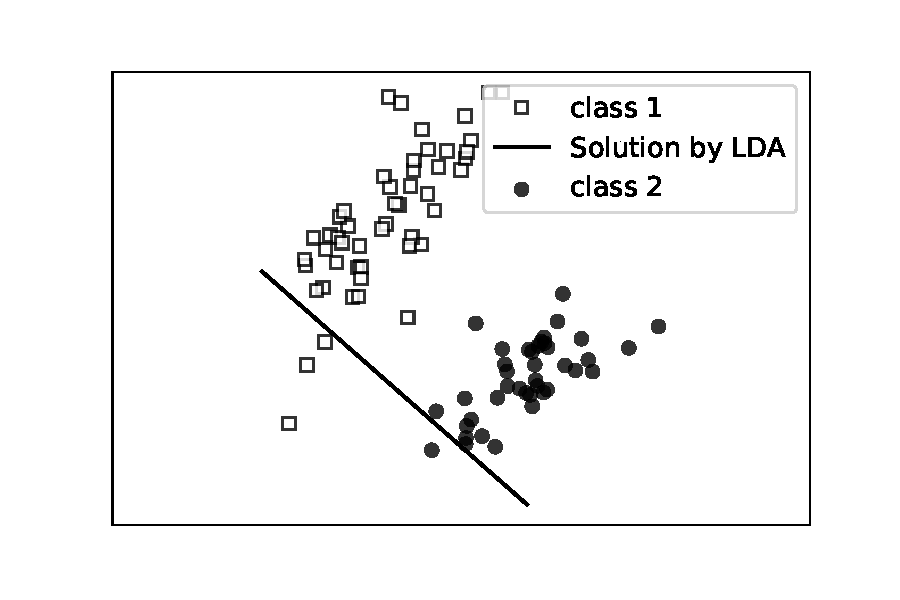
\includegraphics[width=.5\textwidth]{Chapters/07_DimemsionalityReduction/29_lda/python/res.pdf}
    }
\end{figure}
% ******************************************************************************
 
Để kiểm chứng độ chính xác của nghiệm tìm được, ta cùng so sánh nó với nghiệm tìm được bởi thư viện \pythoninline{sklearn}:
% \newpage  
\begin{lstlisting}[language=Python]
from sklearn.discriminant_analysis import LinearDiscriminantAnalysis
X = np.concatenate((X0, X1))
y = np.array([0]*N0 + [1]*N1)
clf = LinearDiscriminantAnalysis()
clf.fit(X, y)

print('w_sklearn = ', clf.coef_[0]/np.linalg.norm(clf.coef_)) # normalize
\end{lstlisting}
 
\begin{lstlisting}[language=Python]
w_sklearn =  [ 0.75091074 -0.66040371]
\end{lstlisting}
 
Nghiệm tìm theo công thức và nghiệm tìm theo thư viện là như nhau. 
 
Một ví dụ khác so sánh PCA và LDA có thể được tìm thấy tại \textit{Comparison of LDA
and PCA 2D projection of Iris dataset} (\url{https://goo.gl/tWjAEs}). 
 
\newpage
\section{Thảo luận}

\begin{itemize}
    \item LDA là một phương pháp giảm chiều dữ liệu có sử dụng thông tin về
    label của dữ liệu. Vì vậy, LDA là một thuật toán học có giám sát. 
     
    \item Ý tưởng cơ bản của LDA là tìm một không gian mới với số chiều nhỏ hơn
    không gian ban đầu sao cho hình chiếu của các điểm trong cùng lớp trong không gian mới gần nhau trong khi hình chiếu của các điểm thuộc các lớp khác
    nhau xa nhau. 
     
    \item Trong PCA, số chiều của không gian mới có thể là bất kỳ số nào không lớn hơn số chiều và số điểm dữ liệu. Trong LDA, với bài toán có $C$
    lớp, số chiều của không gian mới không được vượt quá $C-1$.
     
    % \item LDA có giả sử ngầm rằng dữ liệu của các lớp đều tuân theo phân phối
    % chuẩn và các ma trận hiệp phương sai của các classes là gần nhau. 
    \index{tách biệt tuyến tính -- linearly separable}
    \item Với bài toán có hai lớp, từ Hình~\ref{fig:29_1} có thể thấy rằng
    hai lớp
    là tách biệt tuyến tính khi và chỉ khi tồn tại một đường thẳng và một điểm
    trên đường thẳng đó sao cho dữ liệu hình chiếu của hai lớp nằm về hai phía khác nhau của điểm đó.
     
    \item LDA hoạt động rất tốt nếu các lớp là tách biệt tuyến tính. Chất lượng mô
    hình giảm đi rõ rệt nếu các lớp không tách biệt tuyến tính. Điều này dễ
    hiểu vì dữ liệu chiếu lên mọi phương vẫn bị chồng lần, và việc
    tách biệt không thể thực hiện được như ở không gian ban đầu.
     
    \item Mặc dù LDA có nhiều hạn chế, ý tưởng về phương sai nội lớp nhỏ và phương sai liên lớp lớn được sử dụng rất nhiều trong các
    thuật toán phân loại~\cite{vu2016fast,vu2016learning,Meng2011FDDL}.
 
\end{itemize}
 
